\documentclass[border=3pt]{standalone}
% Shared preamble for every generated figure.
% Matches the report: newtx (Times), greyscale, square boxes.
\usepackage{newtxtext,newtxmath}
% newtx's typewriter (txtt) draws a slashed zero; use Latin Modern instead.
\renewcommand{\ttdefault}{lmtt}
\usepackage{tikz}
\usetikzlibrary{positioning,arrows.meta,calc,fit,backgrounds,shapes.geometric,
                decorations.pathreplacing,decorations.pathmorphing,matrix,patterns}

\definecolor{figgrey}{gray}{0.88}
\definecolor{figmid}{gray}{0.60}
\definecolor{figdark}{gray}{0.35}

\tikzset{
  fig/.style={font=\small},
  box/.style={draw,thick,minimum height=8mm,minimum width=22mm,align=center,
              inner sep=2pt,font=\small},
  greybox/.style={box,fill=figgrey},
  smallbox/.style={draw,minimum height=6mm,minimum width=16mm,align=center,
                   inner sep=2pt,font=\scriptsize},
  ln/.style={-{Stealth[length=2.2mm,width=1.8mm]},thick},
  lnb/.style={{Stealth[length=2.2mm,width=1.8mm]}-{Stealth[length=2.2mm,width=1.8mm]},thick},
  lbl/.style={font=\scriptsize,inner sep=1.5pt},
  note/.style={font=\scriptsize\itshape,inner sep=1.5pt},
}

\begin{document}
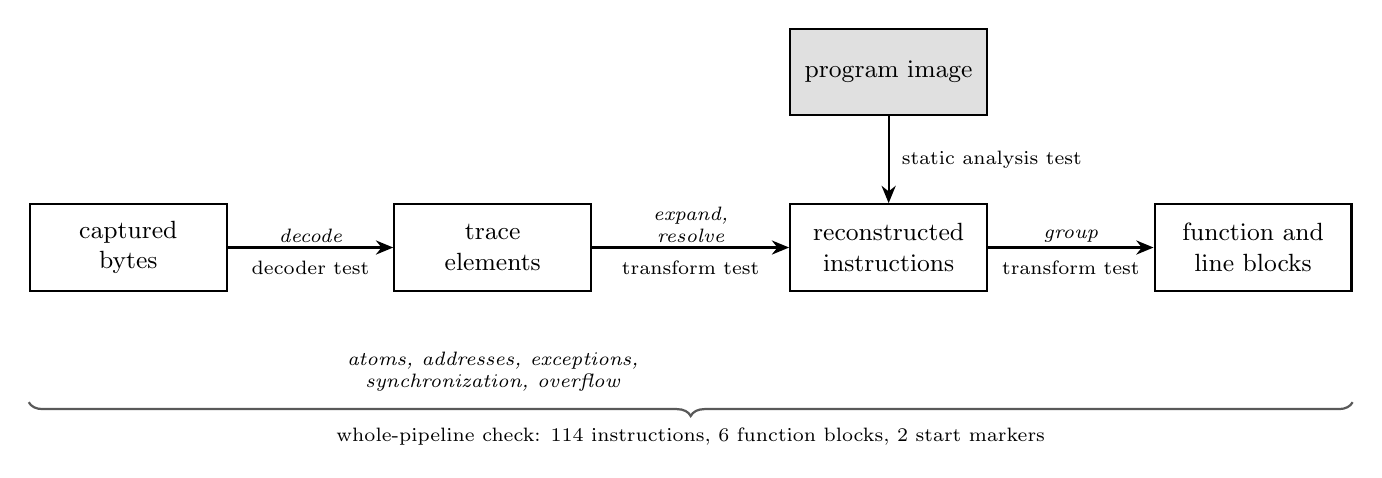
\begin{tikzpicture}[fig,
  st/.style={draw,thick,minimum height=11mm,minimum width=25mm,align=center,font=\small},
  op/.style={font=\scriptsize\itshape,align=center,inner sep=1.5pt},
  tst/.style={font=\scriptsize,align=center,inner sep=1.5pt}]
\node[st] (b) {captured\\bytes};
\node[st,right=21mm of b] (e) {trace\\elements};
\node[st,right=25mm of e] (i) {reconstructed\\instructions};
\node[st,right=21mm of i] (f) {function and\\line blocks};

\draw[ln] (b) -- node[op,above]{decode} node[tst,below=1mm]{decoder test} (e);
\draw[ln] (e) -- node[op,above]{expand,\\resolve} node[tst,below=1mm]{transform test} (i);
\draw[ln] (i) -- node[op,above]{group} node[tst,below=1mm]{transform test} (f);

\node[op,below=7mm of e] {atoms, addresses, exceptions,\\synchronization, overflow};

\node[st,fill=figgrey,above=11mm of i] (img) {program image};
\draw[ln] (img) -- node[tst,right=1mm]{static analysis test} (i);

\draw[decorate,decoration={brace,amplitude=5pt,mirror},figdark,thick]
   ($(b.south west)+(0,-14mm)$) -- ($(f.south east)+(0,-14mm)$);
\node[tst,below=2pt] at ($(b.south west)!0.5!(f.south east)+(0,-16mm)$)
   {whole-pipeline check: 114 instructions, 6 function blocks, 2 start markers};
\end{tikzpicture}
\end{document}
